\documentclass[12pt]{article}

\usepackage[a4paper,margin=1in]{geometry}
\usepackage{setspace}
\onehalfspacing

\usepackage{amsmath,amssymb,amsthm}
\usepackage{graphicx}
\usepackage{float}
\usepackage{caption}
\usepackage{subcaption}
\usepackage{enumitem}
\usepackage{makecell}
\usepackage{booktabs}
\usepackage{hyperref}

% \begin{figure}[htbp]
%     \centering
%     
\includegraphics[width=0.6\textwidth]{hw1_q2b_surface.png}
%     \caption{Optimal joint density f(p, d)}
%     \label{fig:2b}
% \end{figure}

\title{ECON 5345 Homework 6 Report}
\author{Harlly Zhou}
\date{\today}

\begin{document}

\maketitle

\section*{Question 1}
\begin{enumerate}[label=\alph*.]
    \item Since $\Omega$ has a Cholesky decompositive, it is of full rank, denoted by $n$. Then
    \begin{align*}
        \operatorname{rank}(\Omega) = \operatorname{rank}(C'C) = \operatorname{rank}(C) = n.
    \end{align*}
    Since $C$ is full rank, it is invertible.

    \item Taking variance of $e_t$ gives
    \begin{align*}
        CC' = \Omega = \operatorname{Var}(e_t) &= \operatorname{Var}(D(0)v_t)\\
        &= D(0) \operatorname{Var}(v_t) D(0)'\\
        &= D(0) D(0)'.
    \end{align*}
    Therefore, $R = C^{-1} D(0) = C'[D(0)']^{-1}$. It follows that
    \begin{align*}
        RR' = C'[D(0)']^{-1} D(0)(C')^{-1} = I.
    \end{align*}

    \item It is immediate from simple linear algebra:
    \begin{align*}
        R_O(\theta)
        \begin{bmatrix}
            1 & 0 \\
            0 & -1
        \end{bmatrix} = \begin{bmatrix}
            \cos (\theta) & -(-\sin (\theta)) \\
            \sin (\theta) & -\cos (\theta)
        \end{bmatrix}
        = R_E(\theta).
    \end{align*}
    Define $J= \begin{bmatrix}
        1 & 0 \\
        0 & -1
    \end{bmatrix}$. Note that $J$ only flips the sign of the second shock. Suppose $R = R_E(\theta)$. Then we have
    \begin{align*}
        e_t = C R_E(\theta)v_t = C R_O(\theta) J^{-1} v_t.
    \end{align*}
    We can redefine the strutural shock to be $J^{-1} v_t$, and that is WLOG since the identification is up to signs.
\end{enumerate}

\newpage
\section*{Question 2}
Data from 1948Q1 to 2025Q4.
\begin{enumerate}[label=\alph*.]
    \item Up to lag 12, the BIC values are reported in the following table.
    \begin{table}[H]
        \centering
        \caption{BIC for lag order selection}
        \label{tab:q2a_bic}
        \begin{tabular}{cc}
            \toprule
            Lag & BIC \\
            \midrule
            1 & $-10.6600$ \\
            2 & $-10.7058$ \\
            3 & $-10.6398$ \\
            4 & $-10.5738$ \\
            5 & $-10.5274$ \\
            6 & $-10.4613$ \\
            7 & $-10.4023$ \\
            8 & $-10.3386$ \\
            9 & $-10.2701$ \\
            10 & $-10.2099$ \\
            11 & $-10.1462$ \\
            12 & $-10.0781$ \\
            \bottomrule
        \end{tabular}
    \end{table}
    BIC is minimized at lag $p = 2$, so we select $p = 2$.

    \item The long-run restriction is that the demand shock has no long-run effect on output. The estimated matrix is
    \begin{align*}
        \hat{A} = \begin{bmatrix}
            0.008737 & 0.005312 \\
            -0.620508 & 0.139930
        \end{bmatrix}.
    \end{align*}
    This means that a unit of demand shock leads to an increase of 0.008737 unit of output contemporaneously and a decrease of 0.620508 unit of unemployment contemporaneously. A unit of supply shock leads to a increase of 0.005312 unit of output contemporaneously and an increase of 0.139930 unit of unemployment contemporaneously.

    \newpage

    \item The impulse response functions are reported in the following figure. The bootstrap CI is also plotted.
    \begin{figure}[H]
        \centering
        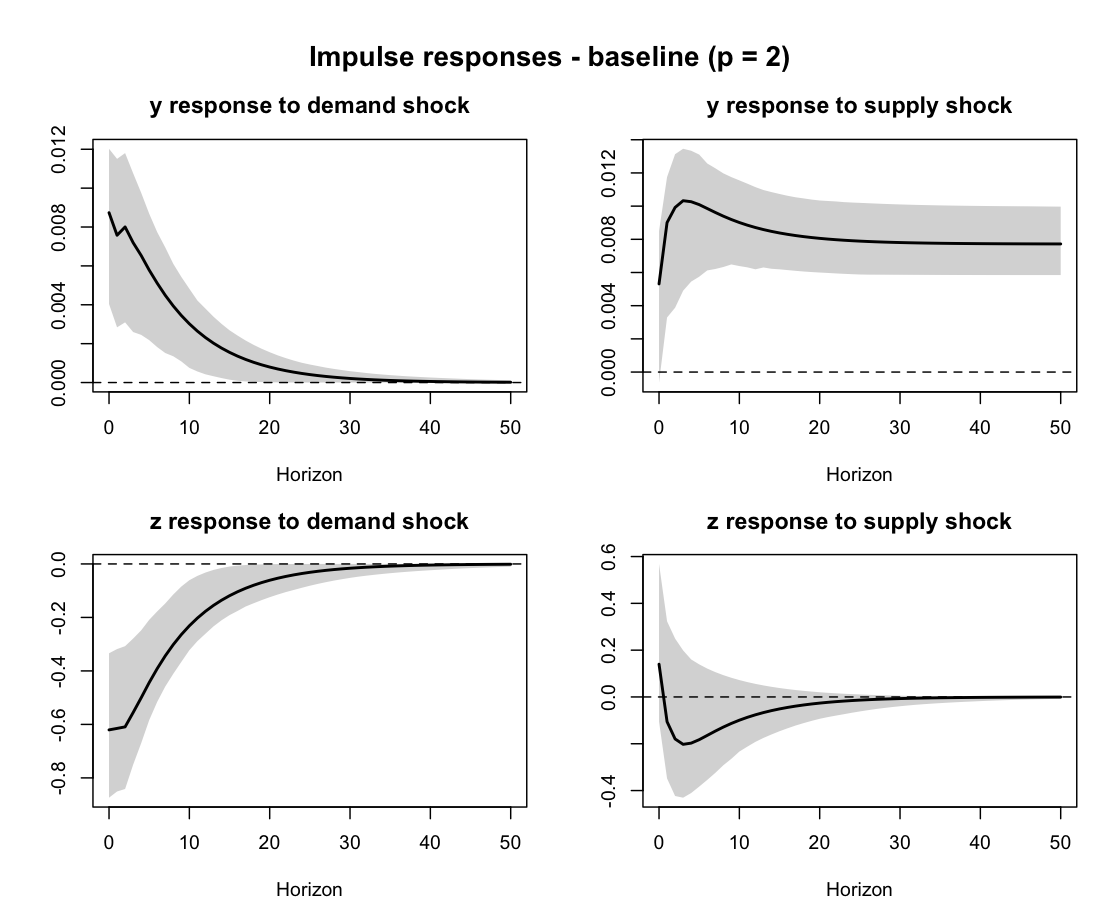
\includegraphics[width=0.8\textwidth]{q2_baseline_irf.png}
        \caption{Impulse response functions: $p=2$}
        \label{fig:q2c_irf}
    \end{figure}
    Output response to demand shock is decreasing over time and converges to zero in the long run, and it is significantly positive. Output response to supply shock converges to a positive constant in the long run, and it is significantly positive. 

    Unemployment response to demand shock is decreasing over time and converges to zero in the long run, and it is significantly negative. Unemployment response to supply shock is not significantly different from zero from the CI, and it converges to zero in the long run.

    \newpage

    \item The FEVD are reported in the following figure.
    \begin{figure}[H]
        \centering
        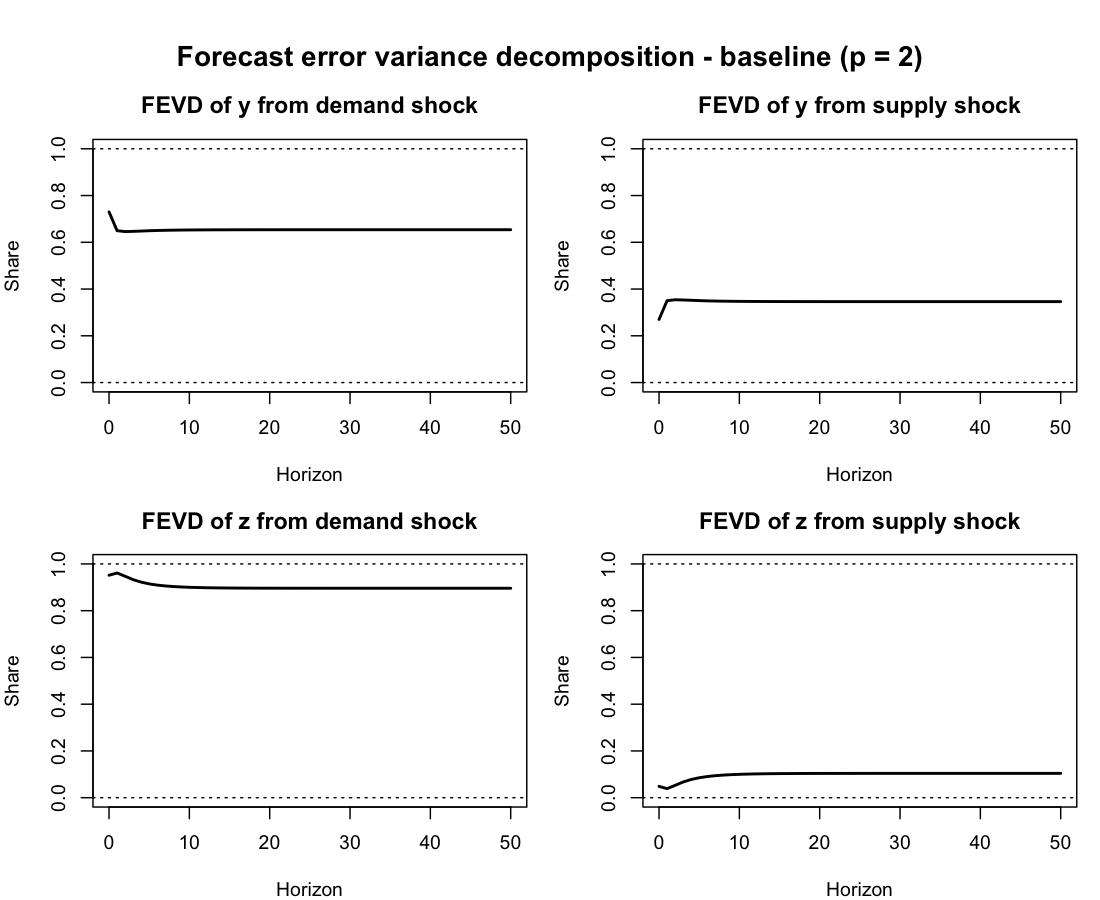
\includegraphics[width=0.8\textwidth]{q2_baseline_fevd.png}
        \caption{Forecast error variance decomposition: $p=2$}
        \label{fig:q2d_fevd}
    \end{figure}

    \item The result is reported in Figure\ref{fig:q2c_irf}.
    
    \newpage
    \item With lag $p=6$, the estimated matrix is
    \begin{align*}
        \hat{A} = \begin{bmatrix}
            0.007332 & 0.007121 \\
            -0.639519 & -0.007545
        \end{bmatrix}.
    \end{align*}
    The IRFs together with the bootstrap CI are reported in the following figure.
    \begin{figure}[H]
        \centering
        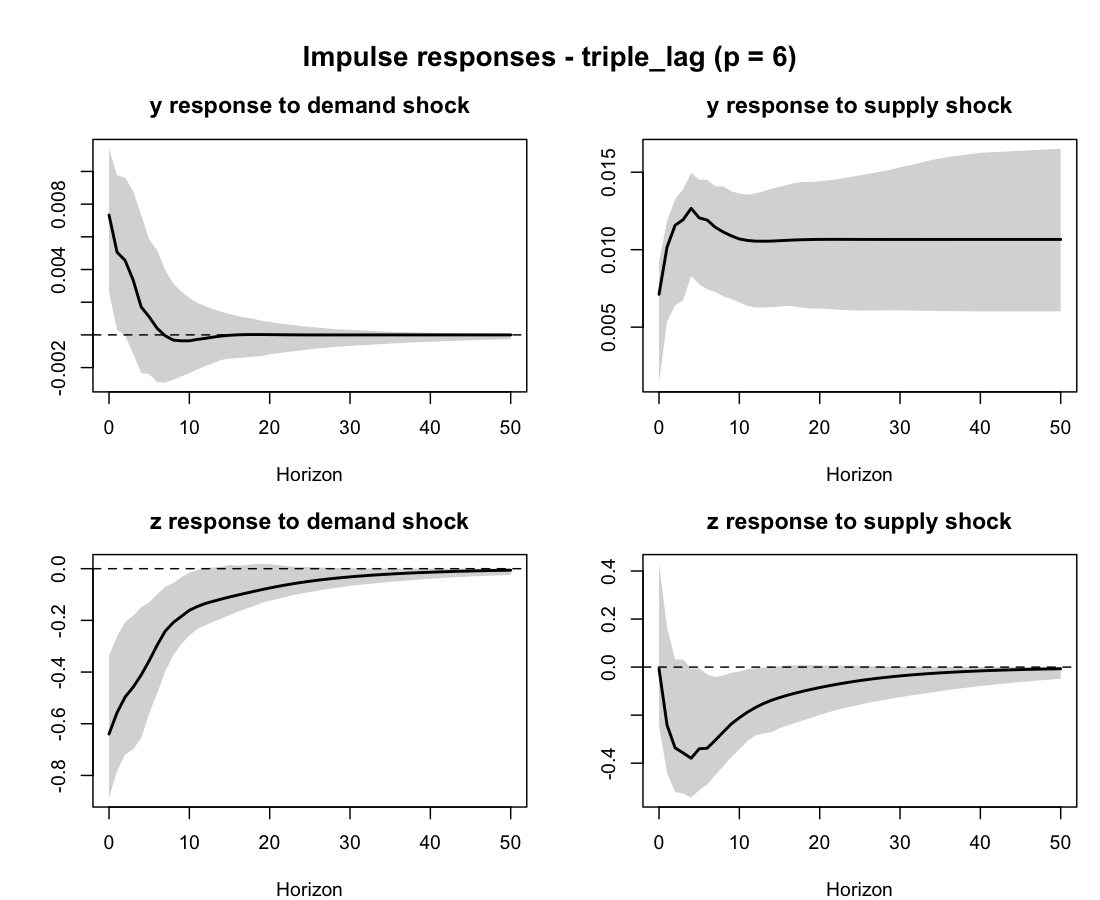
\includegraphics[width=0.8\textwidth]{q2_triple_lag_irf.png}
        \caption{Impulse response functions: $p=6$}
        \label{fig:q2f_irf}
    \end{figure}

    \newpage
    The FEVD are reported in the following figure.
    \begin{figure}[H]
        \centering
        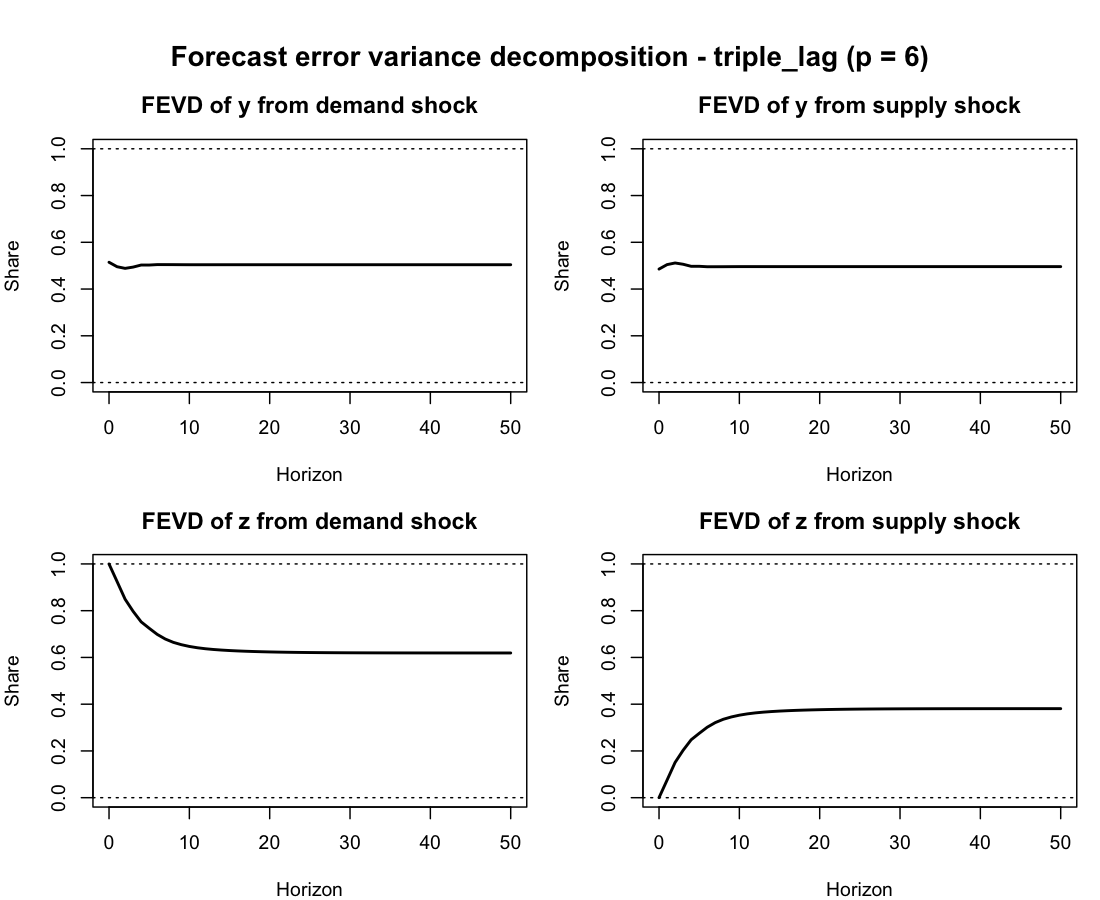
\includegraphics[width=0.8\textwidth]{q2_triple_lag_fevd.png}
        \caption{Forecast error variance decomposition: $p=6$}
        \label{fig:q2f_fevd}
    \end{figure}

    \medskip
    \textbf{Comparison:}
    \begin{itemize}
        \item The contemporaneous effect of supply shock on unemplotment becomes negative. Some medium-run effect may be absorbed by structural demand shocks when the lag length is small. After adding more lags, they are cleared out and the effect becomes negative as purified more.
        \item The responses to demand shock become insignificant more quickly when the lag length is increased from 2 to 6. Same as before, the signficant responses can be medium run autocorrelations.
        \item The output response to supply shock converges to a higher value in the long run when the lag length is increased from 2 to 6. More lags capture more persistent component in output, which contributes to the ouput response to supply shocks.
        \item The unemployment response to supply shock becomes significantly negative after around 1 year when the lag length is increased from 2 to 6. This is consistent with sticky wage models so that the effect on labour market takes time to happen.
        \item The FEV from demand shock on both variables decreases in general when the lag length is increased from 2 to 6. Similarly, the previous high contribution may be medium run autocorrelations.
    \end{itemize}
\end{enumerate}
\end{document}